\documentclass{beamer}
\beamertemplatenavigationsymbolsempty
\usecolortheme{beaver}
\setbeamertemplate{blocks}[rounded=true, shadow=true]
\setbeamertemplate{footline}[page number]
%
\usepackage[utf8]{inputenc}
\usepackage[english]{babel}
\usepackage{amssymb,amsfonts,amsmath,mathtext}
\usepackage{subfig}
\usepackage[all]{xy} % xy package for diagrams
\usepackage{array}
\usepackage{multicol}% many columns in slide
\usepackage{hyperref}% urls
\usepackage{hhline}%tables
% Your figures are here:
\graphicspath{{./fig}}

%----------------------------------------------------------------------------------------------------------
\title[\hbox to 56mm{Feature generation}]{Differential neural ensemble search with diversity control}
\author[P.\,K.~Babkin]{Petr Babkin}
\institute{Moscow Institute of Physics and Technology}
\date{\footnotesize
\par\smallskip\emph{Course:} My first scientific paper\par (Strijov's practice)/Group B05-003
\par\smallskip\emph{Expert:} O.~Bakhteev
\par\smallskip\emph{Consultants:} K.~Yakovlev, K.~Petrushina
\par\bigskip\small 2023}

%----------------------------------------------------------------------------------------------------------
\begin{document}
%----------------------------------------------------------------------------------------------------------
\begin{frame}
\thispagestyle{empty}
\maketitle
\end{frame}
%-----------------------------------------------------------------------------------------------------
\begin{frame}{Goal of research}
..
\end{frame}
%-----------------------------------------------------------------------------------------------------
\begin{frame}{Problem of creating NN ensembles}

    \begin{columns}[c]
    \column{0.4\textwidth}
    Method:
        \begin{enumerate}
            \item find optimal architecture
            \item sample architectures with diversity control
            \item give answer as equal voting
        \end{enumerate}
    \column{0.6\textwidth}
        \begin{figure}
            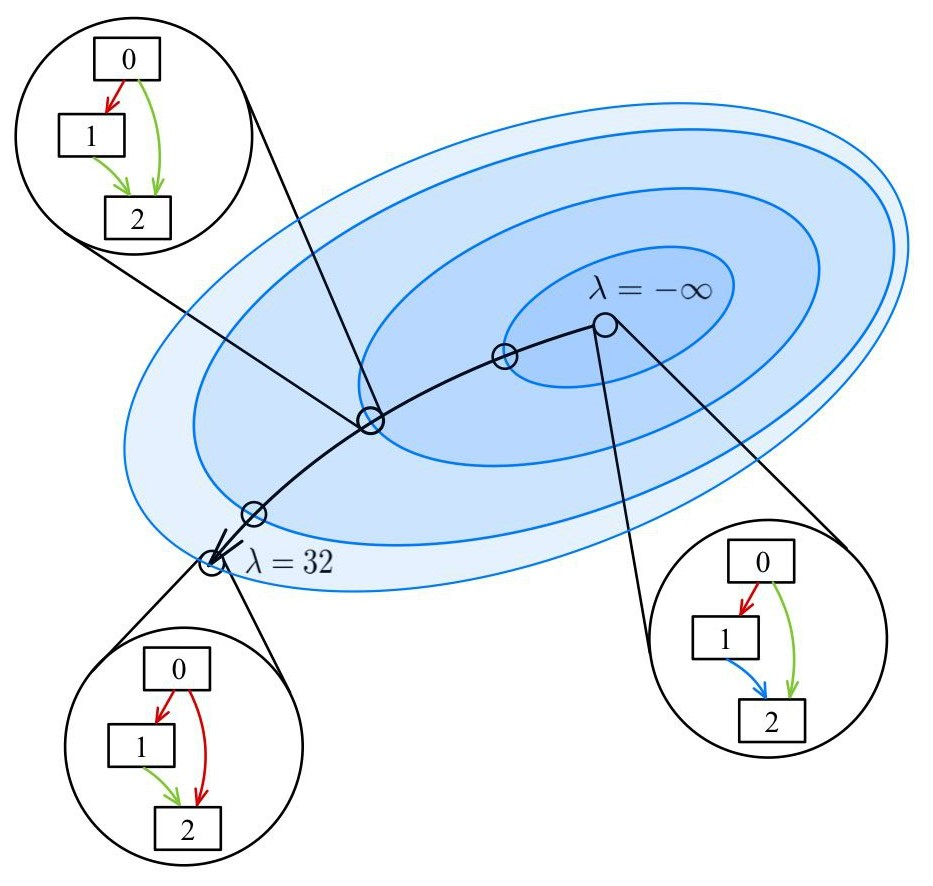
\includegraphics[scale=0.21]{scheme}
        \end{figure}
    \end{columns}

    \bigskip
    Problem of sampling new models for ensemble: 
    \begin{gather*}
        \min_{\alpha} \mathbb{E}_{\lambda \sim U(0, \Lambda)} [\mathcal{L}_{val}(w^*, \alpha(\lambda)) - \lambda JS(\alpha^*, \alpha(\lambda))] \\
        s.t. \text{ } w^* = \arg \min_w \mathbb{E}_{\lambda \sim U(0, \Lambda)}[\mathcal{L}_{train}(w, \alpha(\lambda))]
    \end{gather*}

\end{frame}


%----------------------------------------------------------------------------------------------------------
\begin{frame}{Problem statement}
..
\end{frame}
%----------------------------------------------------------------------------------------------------------
\begin{frame}{Solution}
\begin{columns}[c]
\column{0.6\textwidth}
    Column 1
\column{0.4\textwidth}
    Column 2
\end{columns}
\end{frame}
%----------------------------------------------------------------------------------------------------------
\begin{frame}{Computational experiment}
..
\end{frame}
%----------------------------------------------------------------------------------------------------------
\begin{frame}{Conclusion}
    \begin{block}{Forecast with hierarchical aggregation of}
    \begin{itemize}
        \item types of freight in
        \item stations, regions, and roads,
        \item for a day, week, month, and quarter.
    \end{itemize}
    \end{block}
\end{frame}
%----------------------------------------------------------------------------------------------------------
\end{document} 